\documentclass[11pt, a4paper]{article}
\sloppy %prevents text from going over the right margin
% \usepackage[T1]{fontenc}
\usepackage[utf8]{inputenc}
\usepackage{listings}
\usepackage[margin=1.0in]{geometry}
\usepackage{color}
\usepackage{graphicx}
\usepackage{tabularx}
\usepackage{url}
\usepackage[normalem]{ulem} 
\usepackage{enumitem}
\usepackage{hyperref}
\usepackage{fancyhdr} %Package to configure headings and footer
\usepackage{lastpage}
%\usepackage[ngerman]{babel}
\setlength\parindent{0pt}

\newcommand{\VARtitle}{DEZSYS09}
\newcommand{\VARauthor}{Janeczek}

\title{General Purpose Computing on GPUs \\ \VARtitle}
\author{\VARauthor}
\date{\today{}, Vienna}

% header
\pagestyle{fancy}
\fancyhead[L]{\today}
\fancyhead[R]{\VARtitle}

%footer
\fancyfoot[L]{\VARauthor}
\fancyfoot[C]{5AHITT}
\fancyfoot[R]{Page \thepage/\pageref{LastPage}}


\begin{document}

\lstset{ %
  backgroundcolor=\color{white},   % choose the background color; you must add \usepackage{color} or \usepackage{xcolor}
  basicstyle=\footnotesize,        % the size of the fonts that are used for the code
  breakatwhitespace=false,         % sets if automatic breaks should only happen at whitespace
  breaklines=true,                 % sets automatic line breaking
  captionpos=b,                    % sets the caption-position to bottom
% commentstyle=\color{mygreen},    % comment style
  deletekeywords={...},            % if you want to delete keywords from the given language
  escapeinside={\%*}{*)},          % if you want to add LaTeX within your code
  extendedchars=false,              % lets you use non-ASCII characters; for 8-bits encodings only, does not work with UTF-8
% frame=single,                    % adds a frame around the code
  keepspaces=true,                 % keeps spaces in text, useful for keeping indentation of code (possibly needs columns=flexible)
% keywordstyle=\color{blue},       % keyword style
% language=bash,                   % the language of the code
  morekeywords={*,...},            % if you want to add more keywords to the set
  numbers=left,                    % where to put the line-numbers; possible values are (none, left, right)
  numbersep=5pt,                   % how far the line-numbers are from the code
  rulecolor=\color{black},         % if not set, the frame-color may be changed on line-breaks within not-black text (e.g. comments (green here))
  showspaces=false,                % show spaces everywhere adding particular underscores; it overrides 'showstringspaces'
  showstringspaces=false,          % underline spaces within strings only
  showtabs=false,                  % show tabs within strings adding particular underscores
  stepnumber=1,                    % the step between two line-numbers. If it's 1, each line will be numbered
  tabsize=2,                       % sets default tabsize to 2 spaces
  title=\lstname                   % show the filename of files included with \lstinputlisting; also try caption instead of title
}


\maketitle
\newpage
\tableofcontents
\newpage


\section{Task Description}

GPU Computing oder GPGPU(= General Purpose Computing on GPUs) bezeichnet die Verwendung eines Grafikprozessors (engl. Graphics Processing Unit oder GPU) für allgemeine Berechnungen im wissenschaftlich-technischen Bereich. Übersetzt bedeutet GPGPU in etwa Allgemeine Berechnung auf Grafikprozessoren. \\

Informieren Sie sich über die Möglichkeiten der Nutzung von GPUs in normalen Anwendungen. Zeigen Sie dazu im Gegensatz den Vorteil der GPUs in rechenintensiven Implementierungen auf [1Pkt]. Gibt es Entwicklungsumgebungen und in welchen Programmiersprachen kann man diese nutzen [1Pkt]? Können bestehende Programme (C und Java) auf GPUs genutzt werden und was sind dabei die Grundvoraussetzungen dafür [1Pkt]? Gibt es transcompiler und wie kommen diese zum Einsatz [1Pkt]? \\

Präsentieren Sie an einem praktischen Beispiel den Nutzen dieser Technologie. Wählen Sie zwei rechenintensive Algorithmen (z.B. Faktorisierung) und zeigen Sie in einem Benchmark welche Vorteile der Einsatz der vorhandenen GPU Hardware bringt [12Pkt]! Um auch einen Vergleich auf verschiedenen Platformen zu gewährleisten, bietet sich die Verwendung von OpenCL an. \\

Diese Aufgabe ist als Gruppenarbeit (2) zu lösen. Zusätzliche Abgaben erhöhen die Gesamtpunkte und können somit zur Notenverbesserung dienen. \\

\textbf{Quellen} \\
http://www.nvidia.de/page/gpu\_computing.html \\
http://developer.nvidia.com/cuda-gpus \\
http://people.maths.ox.ac.uk/gilesm/cuda/ \\
http://www.khronos.org/opencl/ \\

\newpage

\section{Requirements Analysis}
\subsection{GPGPU Investigation}
Do a little research on General Purpose Computing on GPUs and find answers to the questions mentioned above.
\subsection{Practical Implementation/Example}
Make use of the GPGPU technology and elaborate two CPU-intensive algorithms. Show which advantages come with using the GPU hardware in shape of a benchmark.

\section{Effort Estimation}
\subsection{Estimated Effort}

\begin{center}
  \begin{tabular}{| l | l |}
		\hline
	    Task & Effort  \\ \hline
		GPGPU Investigation & 3h \\ \hline
	    Implementation and Benchmark  & 5h  \\ \hline 
		Writing the documentation & 1h\\ \hline \hline
		Total & 9h \\ \hline
  \end{tabular}
\end{center}

\subsection{Actual Effort}

\begin{center}
  \begin{tabular}{| l | l |}
		\hline
		Task & Effort  \\ \hline
		GPGPU Investigation & ?h \\ \hline
		Implementation and Benchmark  & ?h  \\ \hline 
		Writing the documentation & ?h\\ \hline \hline
		Total & ?h \\ \hline
  \end{tabular}
\end{center}

\subsection{Apportionment of work}
\begin{center}
  \begin{tabular}{| l | l | l |}
    \hline
    Task & Janeczek & ?  \\ \hline
	GPGPU Investigation &  & ? \\ \hline
	Implementation and Benchmark& x & ? \\ \hline
    Writing the documentation & x  & ?  \\ \hline 
  \end{tabular}
\end{center}

\newpage

\section{Task Execution}
\subsection{Investigation on GPGPU}

\textbf{What is GPU Accelerated Computing?}

\textit{"GPU-accelerated computing is the use of a graphics processing unit (GPU) together with a CPU to accelerate scientific, analytics, engineering, consumer, and enterprise applications. GPUs are accelerating applications in platforms ranging from cars, to mobile phones and tablets, to drones and robots."}\cite{nvidia-whatis-gpuac}\\

\textbf{How do GPUs accelerate applications?}

\textit{"GPU-accelerated computing offers unprecedented application performance by offloading compute-intensive portions of the application to the GPU, while the remainder of the code still runs on the CPU."}\cite{nvidia-whatis-gpuac}\\

\begin{figure}[h!]
	\centering
	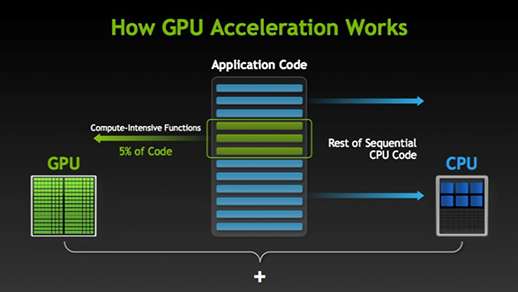
\includegraphics[width=0.8\textwidth]{how-gpu-acceleration-works}
	\caption{An illustration of how GPU acceleration practically works \cite{how-gpu-acc-works}}
\end{figure}

\textbf{CPU versus GPU}

\textit{"A simple way to understand the difference between a CPU and GPU is to compare how they process tasks. A CPU consists of a few cores optimized for sequential serial processing while a GPU has a massively parallel architecture consisting of thousands of smaller, more efficient cores designed for handling multiple tasks simultaneously."}\cite{nvidia-whatis-gpuac}

\begin{figure}[h!]
	\centering
	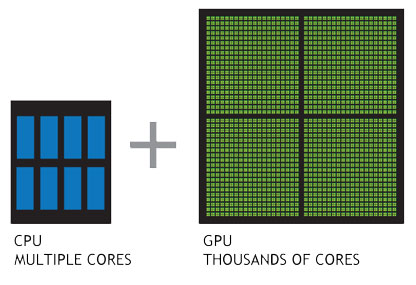
\includegraphics[width=0.4\textwidth]{cpu-and-gpu}
	\caption{GPUs have thousands of cores to process parallel workloads efficiently \cite{cpu-vs-gpu}}
\end{figure}

\newpage
\textbf{Using GPUs in all-day applications}



\newpage
\subsection{RESTful Web Service}
\subsection{Service Oriented Architecture (SOA)}

\newpage
\nocite{*}
\bibliographystyle{plain}
\bibliography{bibliography}{}

\end{document}